\chapter{Introduction}
\label{chapter:intro}

\section{背景與動機}

在人工智慧的浪潮下,已有愈來愈多工廠只餘機器人在工作,人們只需定期去
工廠檢查確保正常營運。科技技術的進步往往能便利人們的生活,也漸漸改變人們生
活的方式,以日常生活舉例,當需要購買生活用品時會去便利超商、量販店或是直
接由網路購物商城購買商品,最近更出現了不須服務人員的無人商店,如:位於西
雅圖的 AmazonGo 無人商店,主打顧客挑選商品完就可以帶著商品離開,不須交由
店員結帳付款,而是自動辨識顧客挑選 的商品進行信用卡扣款,省去了等待排隊
的時間;而網路購物也是相當便利,由廠商針對顧客網路訂單從倉儲進行集貨並由
貨運公司進行運輸到客戶手中,其中許多廠商為了提高集貨的效率已經著手於倉儲
的自動化。然而在無人商店跟倉庫的應用中,現今還無法達成實質無人化,原因是因為如無人商店內商品上架仍需人去逐一整齊擺放,而倉庫在進行商品分類與打包時也須有人去掃描商品條碼才可以知道商品代號和該怎麼打包。這兩者任務雖有所不同,但皆可歸類為需針對商品上語意標籤如品牌文字或條碼去進行套定姿態擺放任務。結合語意標籤進行特定姿勢擺放任務是一較新穎之領域,相當具有挑戰性。便可實際應用於倉庫與無人商店,將可降低大量人力與時間成本。


\section{目標與貢獻}

\subsection{問題定義}
在無人商店與倉庫的許多應用中,夾取與放置任務都十分重要,如無人商店上架必
須放置商品時,品牌文字或商標需朝外放。放置任務尤其以特定姿態放置任務最為困
難,因為其牽涉到物品姿態以及夾取可行性。在此研究中,我將物品表面的一小部分
作為語意標籤, 此語意標籤不僅可以作為物品三維姿態辨識的依據, 更可以做為操作行
為的依據, 物品上可能有不只一個語意標籤如品牌文字、條形碼等, 本研究將專注於再
雜亂環境中,以品牌文字為線索進行特定姿勢放置任務。

\subsection{挑戰}
\begin{itemize}
\item 在雜亂的環境中,產品物件可能互相堆疊,造成物品部分或全部遮蔽 (occlusion)。
由於品牌文字可能只在產品物件的特定平面位置, 也可能在初始位置即被遮蔽,如何偵測品牌文字或是找出品牌文字所在的一面,是本研究重要目標之一
\item 受限於機器手臂與末端效應器(End effector)的工作範圍,即使預測出物體姿態,特定姿態夾取與放置行為仍可能無法執行,或是在移動過程中會遇到障礙物,造成任務失敗。因此假爪的設計與實驗環境的架設,也是本研究的重要議題之一。
\end{itemize}

\subsection{論文貢獻}
\begin{itemize}
\item \textbf{主動式操作搭配雙手臂協作} 除卻被動利用物件辨識與姿態辨識的結果,本論文運用主動式操作概念去改變雜亂場景,去達到對單一物品與品牌文字最佳的的感知能力。本論文提出的方法不僅可以改變相機視角去看到最少遮蔽的品牌文字,也使用雙手臂協作的方式去操作商品,以達到最佳的放置成效。
\item \textbf{建立基準商品語意資料集以訓練與測試模型與演算法效果} 在現今的影像物件分割技術下,訓練一個深度卷積神經網路需要數量龐大且有標註的資料集。
為了訓練物件切割模型,本論文建立了一個資料集,此資料集包含20個物件,且每個物件都有條碼與品牌文字。此資料集包含來自真實世界與虛擬環境的訓練資料以及真實環境的測試集用來評估放置任務的成效。
\end{itemize}

\begin{figure}[ht]
	\centering
	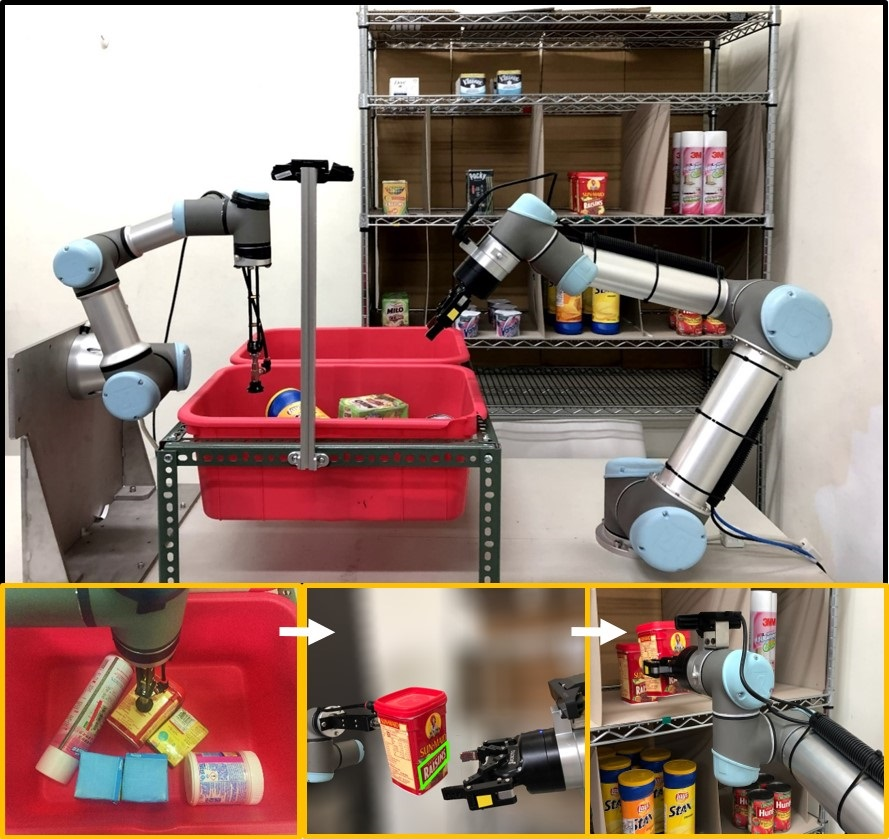
\includegraphics[height=!, width=0.7\linewidth, keepaspectratio=true]
	{./figures/pose-aware-placing-teaser-v3.jpg}
  \caption{本論文利用商品文字(商品上的其中一個語意標籤)作為特殊姿態放置的依據,並設計雙手臂協做的主動式操作系統去解決物品遮蔽的問題。圖左下到右下:吸盤式假爪透過物品或品牌文字語意線索去夾取物品至空曠空間,而兩指式假爪再透過品牌文字線索去執行放置任務。}
  \label{figure:teaser}
\end{figure}

\section{論文架構}
